\section{Event Selection} \label{sec:selection:event_selection}

Starting from the events passing the Large-$R$ trigger discussed in
\Cref{sec:selection:triggers} further selections are made to maximize signal
sensitivity, reject background, and to construct regions where the backgrounds
can be characterized.  First all events are preselected to make sure they
contain at least two large-$R$ jets with $p_{T} > 250\GeV$~\footnote{The 250GeV
cut off was the lowest supported value by the JetEtMiss jet modeling group.}
that also fall entirely within the ID instrumented region $|\eta| < 2.0$ to
make sure charged tracks can be reconstructed for flavor tagging purposes.
Events are further preselected by requiring the leading $p_{T}$ large-$R$ jet
to have $p_{T} > 480\GeV$ and the sub-leading $p_{T}$ large-R jet to have
$p_{T} > 250\GeV$. The leading jet $p_{T}$ cut ensures that all events pass the
offline $p_{T}$ threshold for all three triggers.  The sub-leading jet $p_{T}$
cut is an explicit requirement for the presence of the ISR jet. 

Next the large-$R$ jet assumed to contain the decay products of the Higgs,
refered to as the signal candidate, is selected from the list of large-$R$ jets
passing the following requirements.  The signal candidate must have $p_{T} >
480GeV$ and be sufficiently boosted meaning $p_{T,J} > 2m_{J}$.  It must
contain at least 2 VR track-jets with $p_{T} > 10\GeV$ as required for
$b$-tagging. Furthermore, the distance between the VR track-jets is constrained
by requiring the distance between the two leading VR track-jets ($\Delta
R_{VR}$) to be greater than the radius of the smaller (higher-$p_{T}$) of the
two VR track-jets (min$R_{VR}$).  This requirement helps avoid $b$-tagging
anomalies and prevent signal contamination from gluon splitting.  The highest
$p_{T}$ jet that passes all of the above requirements is labeled the signal
candidate and the next highest $p_{T}$ large-$R$ jet in the list is taken to be
the ISR jet.  Any events containing a muon with $p_{T} > 40\GeV$ opposite the
signal candidate large-$R$ jet, $\Delta \phi > 2\pi/3$, are removed to ensure
no overlap with the $t\bar{t}$ control region ($\text{CR}_t\bar{t}$) discussed
in \Cref{sec:background:ttbar}.  This event selection process is illustrated in
\Cref{fig:event_selection}.

\begin{figure}[!htbp]
  \centering
\begin{tikzpicture}[thick, node distance=2.25cm]
 \node (trigger) [selection] {Trigger \\ 1 large-$R$ jet \\ $p_{T} > 480~\textrm{GeV}$};
 \node (pre) [selection, below of=trigger] {Pre-selection \\ $\geq 2$ large-$R$ jets \\ $p_{T} > 250~\textrm{GeV}$, $|\eta| < 2$};
 \node (signal) [selection, below left of=pre, node distance=4.5cm, fill=blue!30] {\underline{Signal Candidate}\\Boosted\\$\geq2$ VR track jets\\ $\Delta R_{VR}/\mathrm{min} R_{VR} > 1$ \\ Surviving leading \\ $p_{T}$ large-$R$ jet \\ $p_T > 480~\textrm{GeV}$};
 \node (ISR) [selection, below right of=pre, node distance=3.5cm, fill=green!30] {\underline{ISR} \\ Leading $p_{T}$ large-$R$ jet remaining in candidate list};

 \draw [arrow] (trigger) -- (pre);
 \draw [arrow] (pre) -- (signal);
 \draw [arrow] (pre) -- (ISR);
 \node (jet_box) [selection, dashed, minimum width=10.2cm, minimum height=3.7cm, fill=none, below] at (-0.3,-3.6) {};
 \node (jet_box_text) [below right of=jet_box, xshift=1.2cm, yshift=0.1cm] {large-$R$ jet labeling};
\end{tikzpicture}

  \caption{\cite{Feickert:2690521} Diagram of the event selection process and the labeling scheme of the large-$R$ jets in the signal candidate event.}
  \label{fig:event_selection}
\end{figure}

After choosing the signal candidate events they are classified based on how
many of the two leading VR trackjets pass $b$-tagging criteria.  Two
$b$-tagging criteria were used, the ``loose" working point with an 85\%
efficiency and the ``tight" working point with a 77\%
efficiency~\footnote{These working points are determined by applying the
$b$-tagging algorithm to a Monte Carlo sample of $t\bar{t}$ events and then
checking the output against truth information to determine efficiencies.}.
Events with exactly 0 ``loose" $b$-tagged track-jets form the control region
used to estimate the non-resonant QCD background ($\text{CR}_{\text{QCD}}$)
discussed in chapter \Cref{sec:background:qcd}.  Events with exatly 2 ``tight"
$b$-tagged track-jets form the signal region (SR) where the final fit is
perfomed.  The 77\% working point use to form the SR was choosen to optimize
signal significance.  For reference the simulated flavor composition of the SR
is shown in \Cref{fig:selection:flavor_composition}.

\begin{figure}[!htbp]
\centering
\subcaptionbox{(a)\label{fig:selection:flavor_composition}}{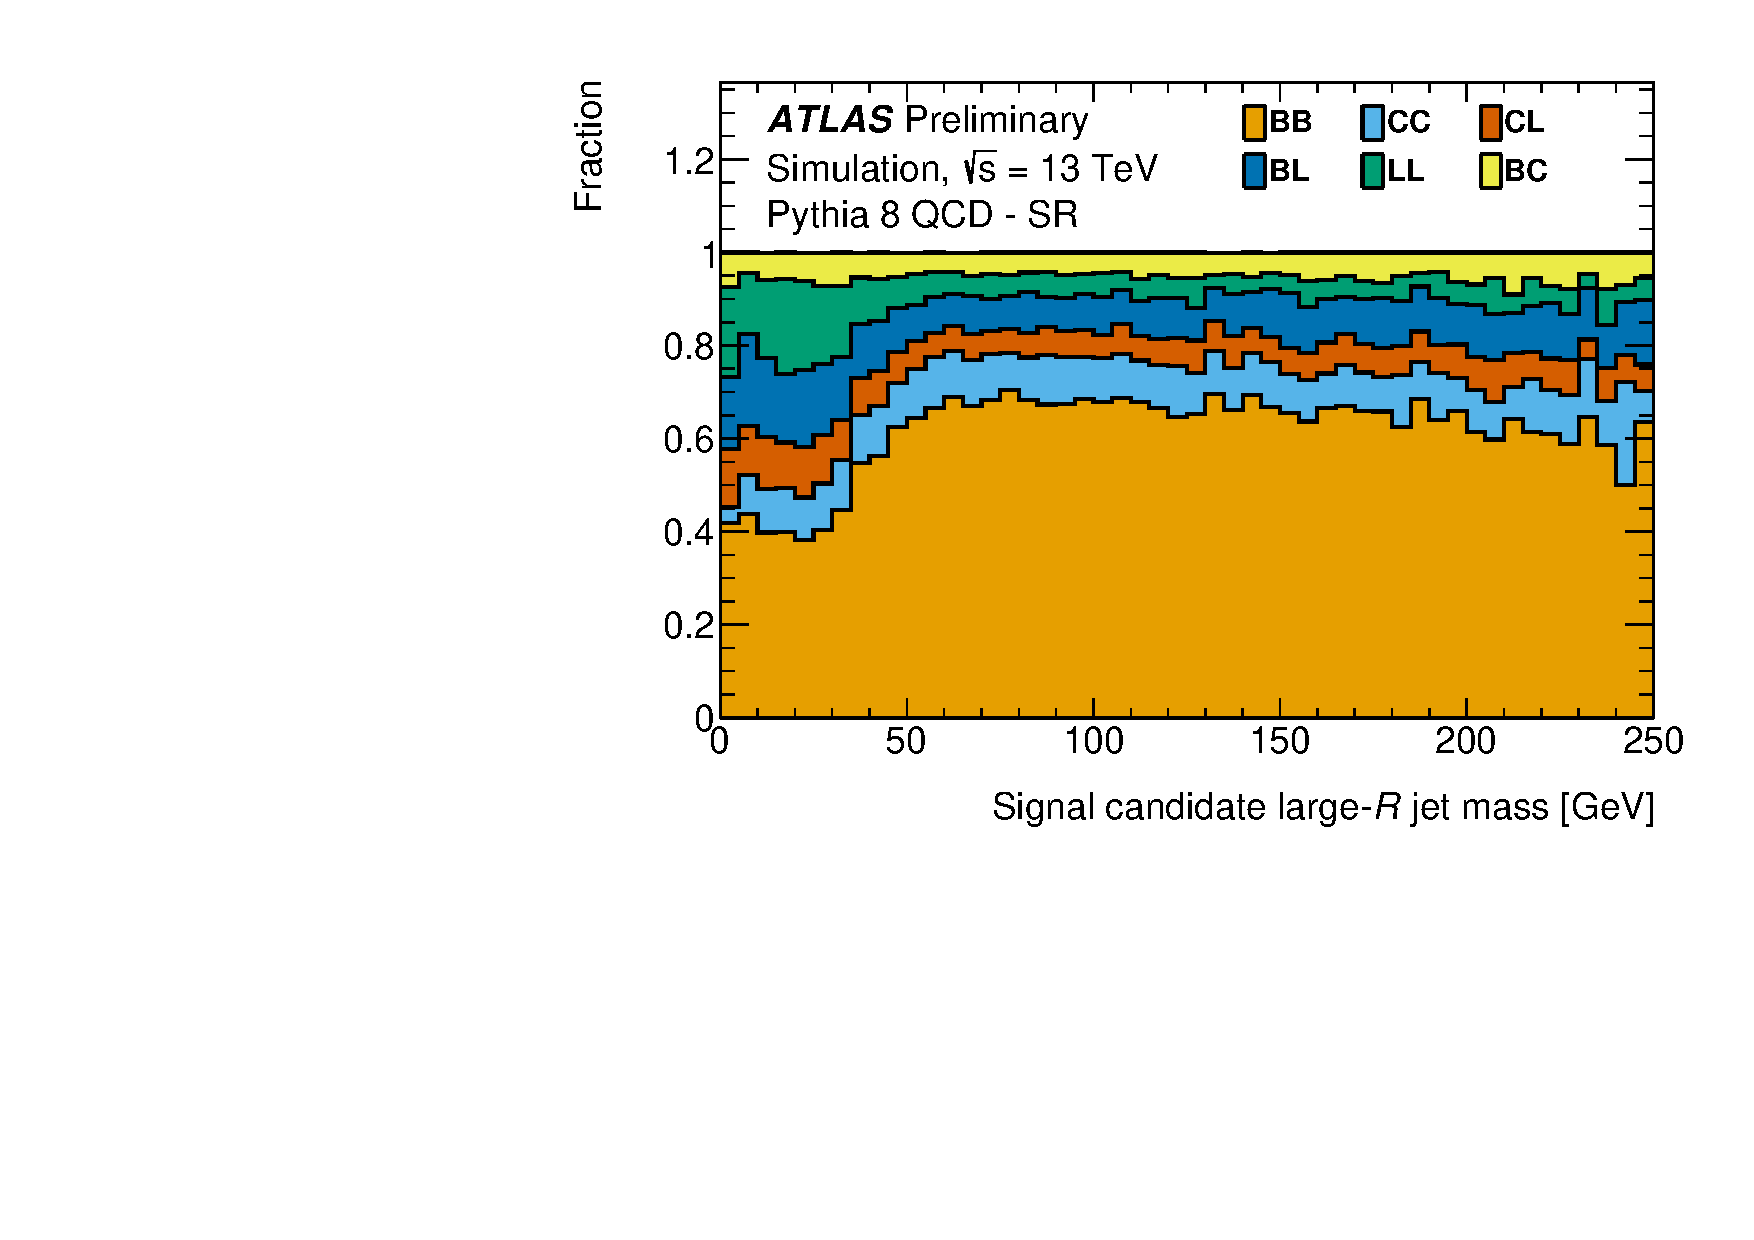
\includegraphics[width=0.48\textwidth]{figures/selection/flavor_composition}}\hfill
\subcaptionbox{(b)\label{fig:selection:sr_cr_shape}}{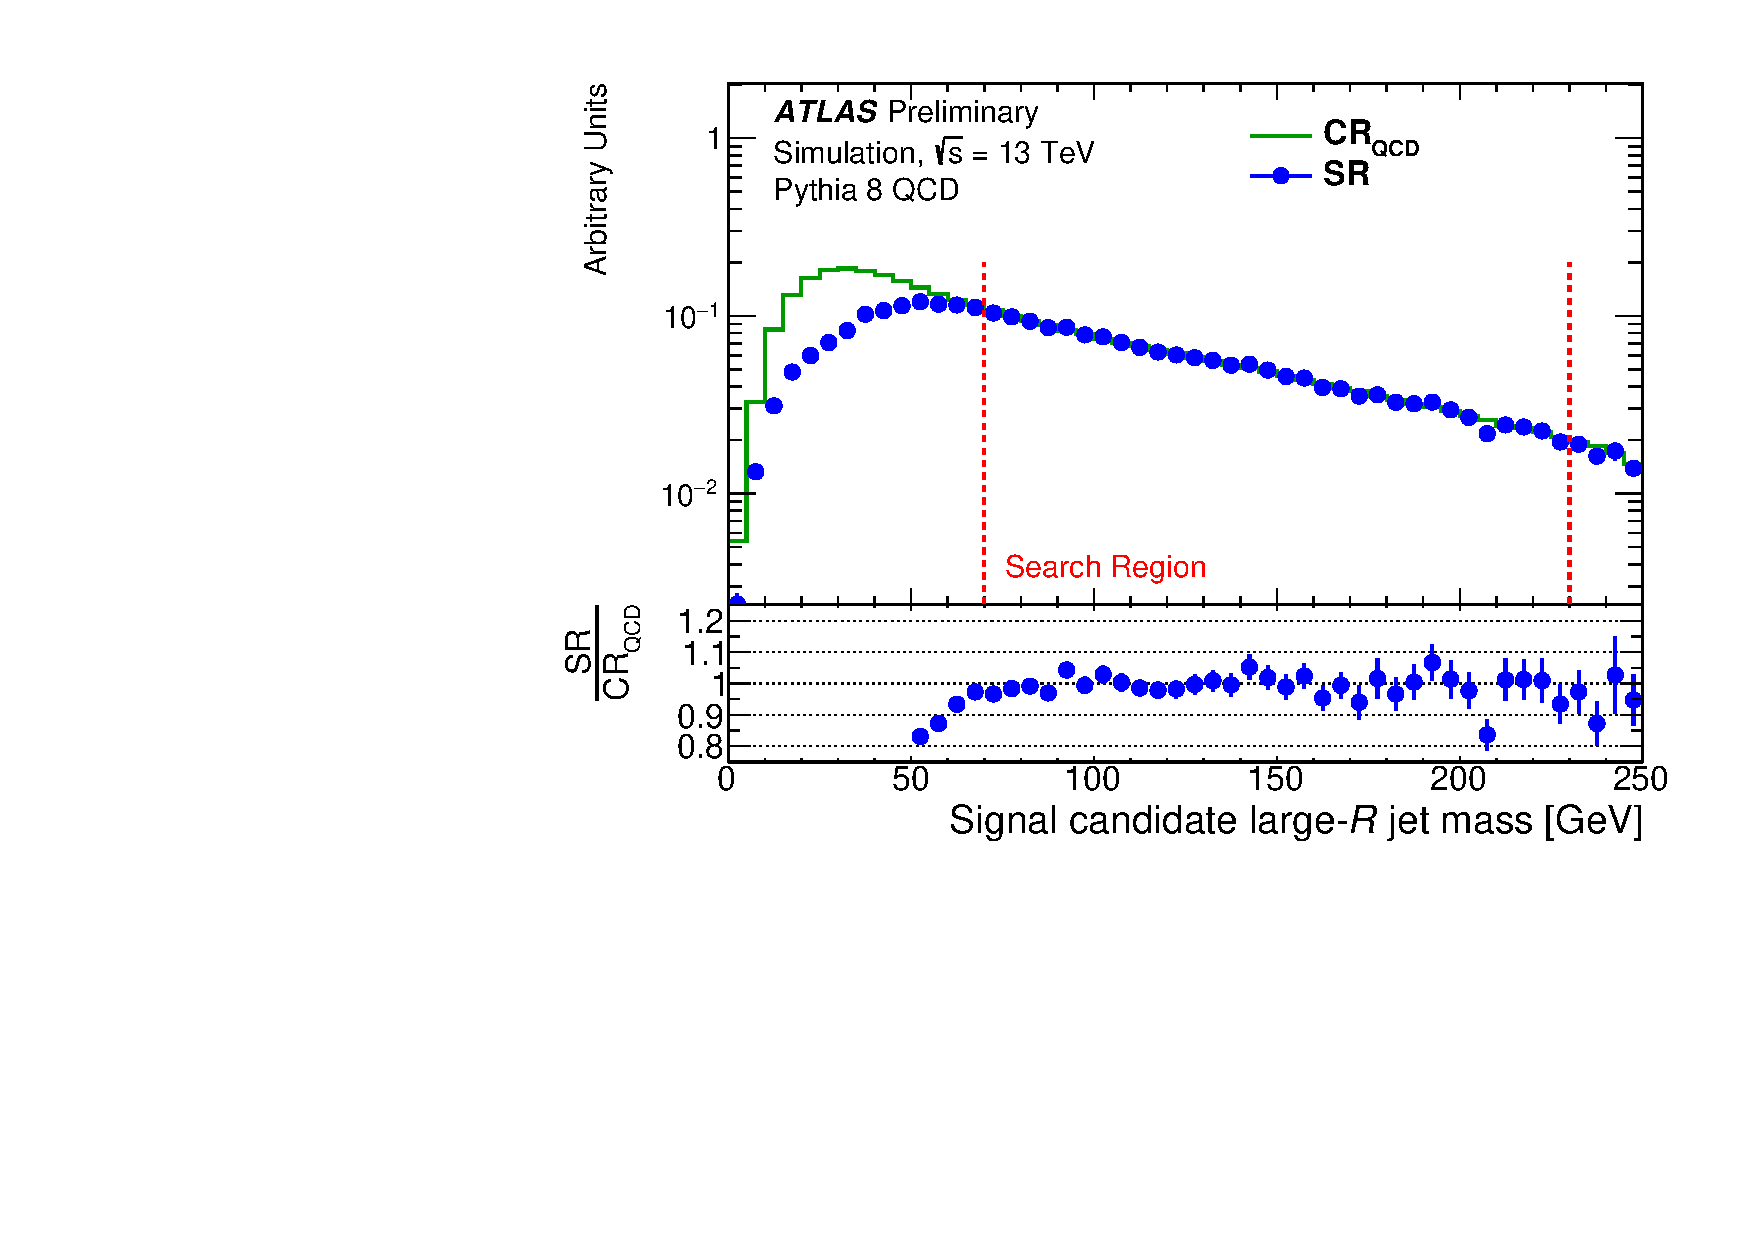
\includegraphics[width=0.48\textwidth]{figures/selection/sr_cr_shape}}

\caption{\cite{ATLAS-CONF-2018-052} (a) Predicted flavour composition of the dijet background in the SR based on the truth-matched hadron content of the two leading-\pt track-jets associated to the signal candidate large-$R$ jet, with the B/C labels indicating the presence of a $b$/$c$-quark and L indicating the presence of a light quark or a gluon. (b) The expected shape of the dijet background in the SR and CR normalised to the same event count between $70~\GeV < m_{\text{J}} < 230~\GeV$.}
\label{fig:event_selection}
\end{figure}

The QCD estimate is only valid for regions where the SR and
$\text{CR}_{\text{QCD}}$ have a similar dijet mass shape.  This results in a
lower bound cut on the signal candidate mass of $m_{\text{J}} > 70\GeV$ due to
the higher turn on curve of the SR shown in \Cref{fig:selection:sr_cr_shape}.
Furthermore, for $m > 230\GeV$ the boost from a $p_{T}$ of $480\GeV$ is no
longer sufficient to merge two hadrons into a single large-$R$ jet.  Thus the
SR signal candidate mass range considered in the analysis spans from $70~\GeV$
to $230~\GeV$.

Given the above criteria the efficiencies and yields in the SR and
$\text{CR}_{\text{QCD}}$ for the considered resonant backgrounds and the Higgs
signal are shown in \Cref{table:efficiencies_and_yields}. The composition of vector boson, $t\bar{t}$ and $H
\rightarrow b\bar{b}$ resonant components of the SR and
$\text{CR}_{\text{QCD}}$ are given in \Cref{table:fractional_composition}. For the vector boson background
the $W+\text{jets}$ contribution dominates in the $\text{CR}_{\text{QCD}}$ due to its
larger cross section.  However, in the SR the $Z+\text{jets}$ dominates as the $Z$
boson can decay to two $b$-quarks while the $W$ boson cannot.  The $t\bar{t}$
contribution is roughly the same in the SR and $\text{CR}_{\text{QCD}}$ with
$\sim 60\%$ of events decaying entirely to hadrons (All Hadronic), $\sim 40\%$
where one top decays leptonically (Semi-leptonic), and a small percentage where
both tops decay leptonically (Dileptonic). In the SR the dominate $H
\rightarrow b\bar{b}$ production mechanism is ggF, contributing 53\% of the
signal, followed by production with 25\% and Higgstrahlung at 22\%. 

\begin{table}[htpb]
 \centering
 \caption{The efficiencies and yields in the $0$-tag control region ($\text{CR}_{\text{QCD}}$) and signal region (SR) for the non-QCD background, the Higgs boson signal and data. The yields in the $\text{CR}_{\text{QCD}}$ are given for the luminosity used for the background estimate of the non-resonant dijet process discussed in \Cref{sec:background:qcd}. The efficiencies are relative to the leading large-$R$ jet $p_{T} > 480~\GeV$ requirement.}
 \begin{adjustbox}{max width=\textwidth}
  \begin{tabular}{@{}lrrrrr@{}}
   \toprule
   Process                             & $\text{CR}_{\text{QCD}}$ Eff. $(\%)$ & $\text{CR}_{\text{QCD}}$ Yield in $1.4~\ifb$ & SR Eff. $(\%)$ & SR Yield in $80.5~\ifb$ \\ \midrule
   $W \to q\bar{q} + \text{jets}$    & $51.3$               & $3810$                       & $0.4$          & $1500$                  \\
   $Z \to q\bar{q} + \text{jets}$    & $46.2$               & $1470$                       & $3.4$          & $6200$                  \\
   $t\bar{t}$                          & $25.9$               & $1929$                       & $2.5$          & $10550$                 \\
   $H \rightarrow b\bar{b}$                              & $24.3$               & $5$                          & $17.9$         & $216$                   \\
   \phantom{$H \rightarrow b\bar{b}$\quad}~ggF           & $23.6$               & $2$                          & $19.4$         & $115$                   \\
   \phantom{$H \rightarrow b\bar{b}$\quad}~VBF           & $15.8$               & $1$                          & $20.7$         & $53$                    \\
   \phantom{$H \rightarrow b\bar{b}$\quad}~$WH$          & $32.4$               & $1$                          & $12.0$         & $26$                    \\
   \phantom{$H \rightarrow b\bar{b}$\quad}~$ZH$          & $30.5$               & $1$                          & $15.8$         & $21$                    \\
   Data                                & $38.7$               & $519710$                     & $0.6$          & $484600$                \\
   \bottomrule
  \end{tabular}
 \end{adjustbox}
 \label{table:efficiencies_and_yields}
\end{table}

\begin{table}[htpb]
 \centering
 \caption{The fractional composition of the different resonant contributions in the $0$-tag control region ($\text{CR}_{\text{QCD}}$) and the signal region (SR). The fraction is evaluated using the given contribution type as the total.}
 \begin{tabular}{@{}lrr@{}}
  \toprule
  Process                                   & $\text{CR}_{\text{QCD}}$ Fraction & SR Fraction \\ \midrule
  $V+\text{jets}$                                  &                   &             \\
  \phantom{$V+\text{jets}$\quad} $Z+\text{jets}$ & $0.28$            & $0.80$      \\
  \phantom{$V+\text{jets}$\quad} $W+\text{jets}$ & $0.72$            & $0.20$      \\
  $t\bar{t}$                                &                   &             \\
  \phantom{$t\bar{t}$\quad} Hadronic        & $0.58$            & $0.63$      \\
  \phantom{$t\bar{t}$\quad} Semi-leptonic   & $0.38$            & $0.34$      \\
  \phantom{$t\bar{t}$\quad} Dileptonic      & $0.04$            & $0.03$      \\
  $H \rightarrow b\bar{b}$                                    &                   &             \\
  \phantom{$H \rightarrow b\bar{b}$\quad} ggF                 & $0.50$            & $0.53$      \\
  \phantom{$H \rightarrow b\bar{b}$\quad} VBF                 & $0.17$            & $0.25$      \\
  \phantom{$H \rightarrow b\bar{b}$\quad} $WH$                & $0.21$            & $0.12$      \\
  \phantom{$H \rightarrow b\bar{b}$\quad} $ZH$                & $0.12$            & $0.10$      \\
  \bottomrule
 \end{tabular}
 \label{table:fractional_composition}
\end{table}
